\documentclass[a4paper,12pt]{article}

\usepackage{setspace}
\usepackage{xcolor}
\usepackage{graphicx}
\usepackage{geometry}
\usepackage{float}
\usepackage{titlesec}
\usepackage{subfigure}
\usepackage{caption}
\captionsetup{figurewithin=section}
\usepackage{amsmath}
\usepackage{listings}
\usepackage{xcolor}

\begin{document}

\title{\textbf{Homework 2}}
\author{Yunian Pan}
\maketitle{}


\section{Backpropagation}

\subsection{case 1}

Sol: 

Given $x_i = g(y_j) = \dfrac{1}{1+e^{-\sum_j {w_{ji}y_j}}}$, and $\sum_{i}\dfrac{\partial E}{\partial x_i} = -\sum_i {(\dfrac{t_i}{x_i} - \dfrac{1 - t_i}{1 - x_i})}$ apply the chain rule, first take $x_i$ and $y_j$ as fixed to compute the gradient for $w_{ji}$, then take $z_k$ and $y_j$ as fixed to compute the gradient for $w_{kj}$ we have 
\begin{align}
\frac{\partial E}{\partial w_{ji}} & = \frac{\partial E}{\partial x_i}\frac{\partial x_i}{\partial w_{ji}}\nonumber \\
&= (\frac{1-t_i}{1- x_i} - \frac{t_i}{x_i})\frac{\partial g(w_{ji}, y_j) }{\partial w_{ji}} \nonumber \\
& = (\frac{1-t_i}{1- x_i} - \frac{t_i}{x_i}) x^2_i y_{j} e^{-\sum_j{w_{ji}y_j}} \nonumber \\
& = (\frac{1-t_i}{1- x_i} - \frac{t_i}{x_i}) x_i y_{j} (1-x_i) \nonumber \\
& = (x_i - t_i) y_j \nonumber \\
\qquad \nonumber 
\end{align}

\begin{align}
\frac{\partial E}{\partial w_{kj}} & =  \sum_{i} (\frac{\partial E}{\partial x_i}  \dfrac{\partial x_i}{\partial y_j} )\frac{\partial y_j}{\partial w_{kj}} \nonumber \\
& =  \sum_{i} \frac{\partial E}{\partial x_i}(-w_{ji}) x_i (1 - x_i) (-z_k) y_j(1- y_j)\nonumber  \\
& = \sum_{i} \frac{x_i - x_i t_i - t_i + x_i t_i}{ (1-x_i)x_i } (-(-w_{ji}) x_i (1 - x_i))(- (-z_k) y_j(1- y_j)) \nonumber \\
& = \sum_{i} (x_i - t_i) w_{ji} y_j(1- y_j) z_k \nonumber 
\end{align}

Thus, we have\qquad $\sum_{i} \dfrac{\partial E}{\partial w_{ji}} = \sum_i \delta_j^i y_j$, \qquad $\sum_{j} \dfrac{\partial E}{\partial w_{kj}} = \sum_j \delta_k^j z_k$. 

\subsection{case 2}

Sol:

Given the cross-entropy $E = -\sum_i t_i \log(x_i)$ and softmax activation function $x_i = \dfrac{e^{\sum_{j} w_{ji} y_j}}{\sum_{i} e^{\sum_{j} w_{ji}y_j}} = f(w_{11}, \ldots , w_{j1}, \ldots, w_{ji}, \ldots,  w_{jm}, \ldots , y_j, \ldots)$, we have
\begin{align}
\frac{\partial E}{\partial x_i} &= - \frac{t_i}{x_i} \nonumber \\
\quad  \nonumber \\
\frac{\partial x_m}{\partial w_{ji}} & =  \frac{y_j(\delta(i-m) e^{\sum_{j}w_{jm}y_j}( \sum_{i}e^{\sum_{j}w_{ji}y_j} ) - e^{\sum_{j}w_{jm}y_j} e^{\sum_{j}w_{ji}y_j})}{(\sum_{i} e^{\sum_{j} w_{ji}y_j})^2}   \nonumber  \\
& = y_j x_m( \delta(i-m) - x_i)  \nonumber \\
\nonumber \\
\frac{\partial E}{\partial w_{ji}} & = \sum_{m} \frac{\partial E}{\partial x_m} \frac{\partial x_m}{\partial w_{ji}}   \nonumber \\
& = \sum_{m} y_j (-\frac{t_m}{x_m}) x_m( \delta(i - m) - x_i)  \nonumber \\
& = y_j (\sum_{m} t_m \cdot x_i - t_i) \nonumber 
\end{align}
\begin{align}
\frac{\partial E}{\partial w_{kj}} & = \sum_{i}( \sum_{m} (\frac{\partial E}{\partial x_m} \frac{\partial x_m}{\partial y_j}) \frac{\partial y_j}{\partial w_{kj}} ) \nonumber \\
& = \sum_{i} (w_{ji} (\sum_{m} t_m x_i - t_i)) y_j (1 - y_j) z_k \nonumber \\
& =  \sum_{i}(\sum_{m} t_m x_i - t_i)(w_{ji} y_j(1- y_j)) z_k \nonumber
\end{align}
Here\quad$\delta_j^i = \sum_{m} t_m \cdot x_i - t_i$,\quad$\delta_k^j =  \sum_{i}(\sum_{m} t_m x_i - t_i)(w_{ji} y_j(1- y_j))$. 

\section{Vowpal Wabbit}

Data format: there are one example per line in the train/test file, each formatted as [label] $|$ [features], where $label \in \{1,\ldots,26\}$, 
$feature \in R^{617}$, features are expressed as $n: x_n$, where $n$ is the dimension and $x_n$ is a real number.

\quad \\
VW commands are executed through shell scripts:
\lstset{language=sh,breaklines=true,frame=single,commentstyle=\color{red!50!green!50!blue!50}}
\begin{lstlisting}
    #!/bin/bash

    # creat a loss file to record the training and testing results
    loss_file=oaa_loss.csv
    if [ -e "$loss_file" ]; then
        rm $loss_file
        echo "train/test,learning_rate,passes,average_loss" >>$loss_file
    fi
    
    # loop for training
    for pss in `seq 1 20` # passes up to 20
    do
        for n in `seq -4 0` # learning rate 
        do
            l_rate=`echo "scale=2; 2^$n" | bc -l`
    
            echo -e "*** train; learning rate: 2^$n; passes: $pss.  *** \n"
    
            # train model and save terminal output to train_log.txt
            vw --oaa 26 isolet_train.vw --cache_file cache_train --sgd -l $l_rate --passes $pss -f oaa.model >train_log.txt 2>&1
    
            # extract average train loss using regular expression
            avg_loss=`cat train_log.txt | grep "average loss = " | grep -o -E "([0-9]+.[0-9]+)|((\+|-)nan)"`
            echo "train,${l_rate},${pss},${avg_loss}" >>$loss_file
    
            echo -e "*** test *** \n"
    
            # test model and save terminal output to test_log.txt
            vw -t -c isolet_test.vw -i oaa.model >test_log.txt 2>&1
            
            # extract average test loss using regular expression
            avg_loss=`cat test_log.txt | grep "average loss = " | grep -o -E "[0-9]+.[0-9]+"`
            echo "test,${l_rate},${pss},${avg_loss}" >>$loss_file
    
        done
    done
    
    rm test_log.txt train_log.txt 
\end{lstlisting}


For ect model we can change the keyword 'oaa' into 'ect'. the script for one-against-all model iteratively(from 1 to 20 passes and different learning rates) executes vw training commands:
\lstset{language=sh,breaklines=true,frame=single,commentstyle=\color{red!50!green!50!blue!50}}
\begin{lstlisting}
 vw --oaa 26 isolet_train.vw -c --sgd -l $l_rate --passes $pss -f oaa.model >train_log.txt 2>&1
\end{lstlisting}
which use SGD as the solver, parameter $l\_rate$ as the learning rate, $pss$ as the passes to train an one-against-all model extracted to the binary file $oaa.model$, 
with all the results output to a log file $train\_log.txt$, then the script uses regular expression to parse the average losses, learning rates and passes and output them to loss file $oaa\_loss.csv$. During
each loop, after trainning the script does VW commands:
\lstset{language=sh,breaklines=true,frame=single,commentstyle=\color{red!50!green!50!blue!50}}
\begin{lstlisting}
    vw -t -c isolet_test.vw -i oaa.model >test_log.txt 2>&1
\end{lstlisting}
which test $oaa.model$ on the test data $isolet\_test.vw$ and save the terminal output to file $test\_log.txt$, then the scripts parses the results into loss file.

After the steps above, I could find the minimum in $oaa\_loss.csv$ and $ect\_loss.csv$, in the first place I tried learning rates $\{0.001, 0.01, 0.1,  1\}$,
and it turned out setting 0.1 has the best performance of all passes settings:
\begin{figure}[htbp]
    \centering
    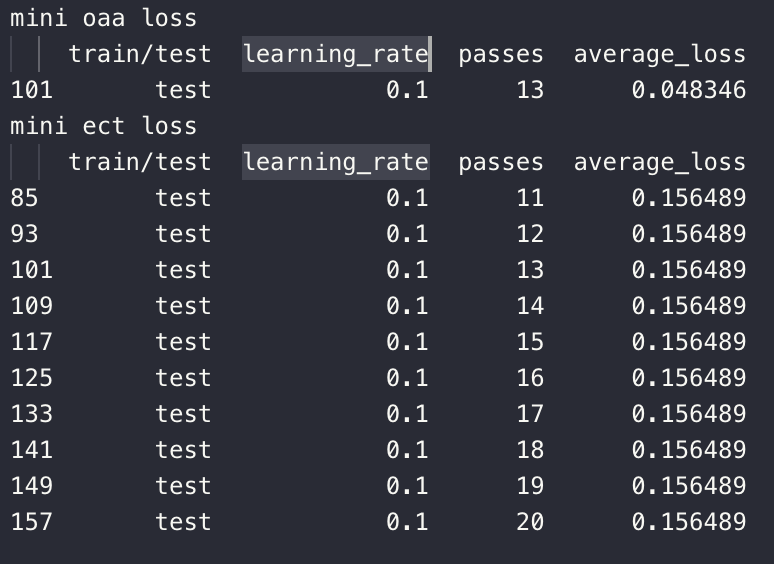
\includegraphics[width = .5\textwidth]{first_result}
\end{figure}

Therefore I explored several different learning rate settings around the neighbor of 0.1, using $learning \ rate = 2^n$ with $n$ from -4 to 0:
\begin{figure}[htbp]
    \centering
    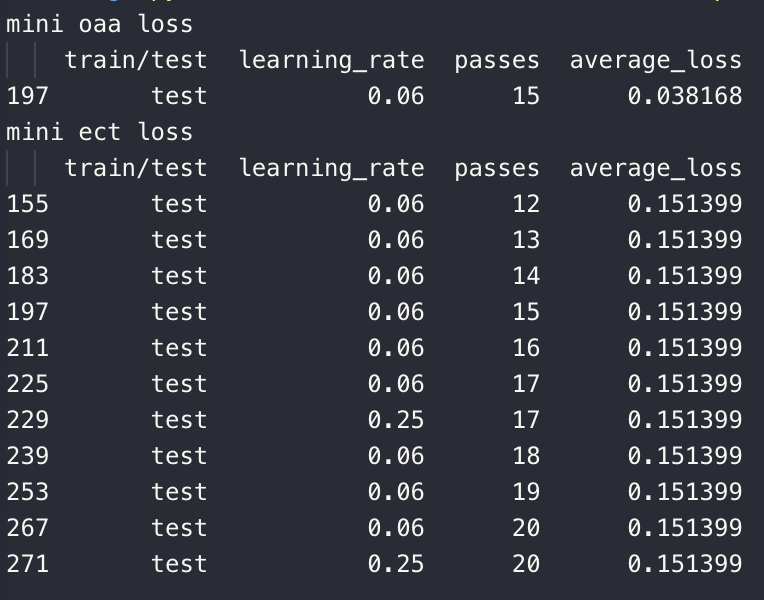
\includegraphics[width = .5\textwidth]{result}
\end{figure}
To summarize, the oaa model performs better than ect model on this dataset, with its minimum loss being around 0.04, the ect reaches its minimum loss around 0.15 after
passes increased to 11 or 12, 0.06 is generally better than other learning rate settings, while the best passes setting is around 15.



\section{Classification}

The network is shown in $\ref{net1}$, each hidden layer has 20 Relu nodes,
\begin{figure}[htbp]
    \centering
    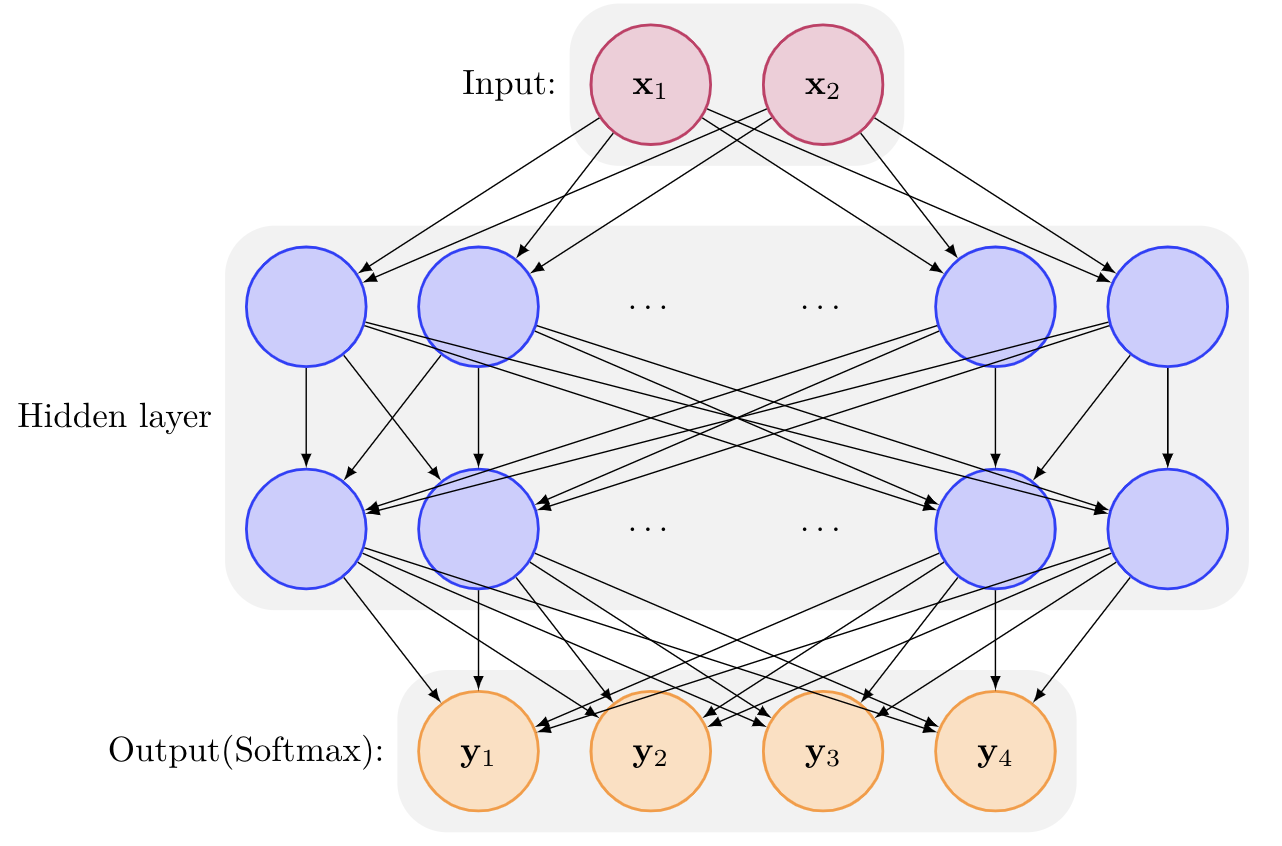
\includegraphics[width = .65\textwidth]{net1}
    \caption{fc-net}
    \label{net1}
\end{figure} 

Each of the output nodes assigns a probability value computed through softmax,
we choose the dimension of maximum probability as prediction of the multi-class, the log-likelihood loss is
setting learning rate as $0.01$, using momentum SGD with batch size = 10 and momentum = 0.5, 
after 10 epoch we can get following results as shown in $\ref{res3}$, with average test and train loss being around 0.2 and both accuracy being around $92\%$.
\begin{figure}[htbp]
    \centering
    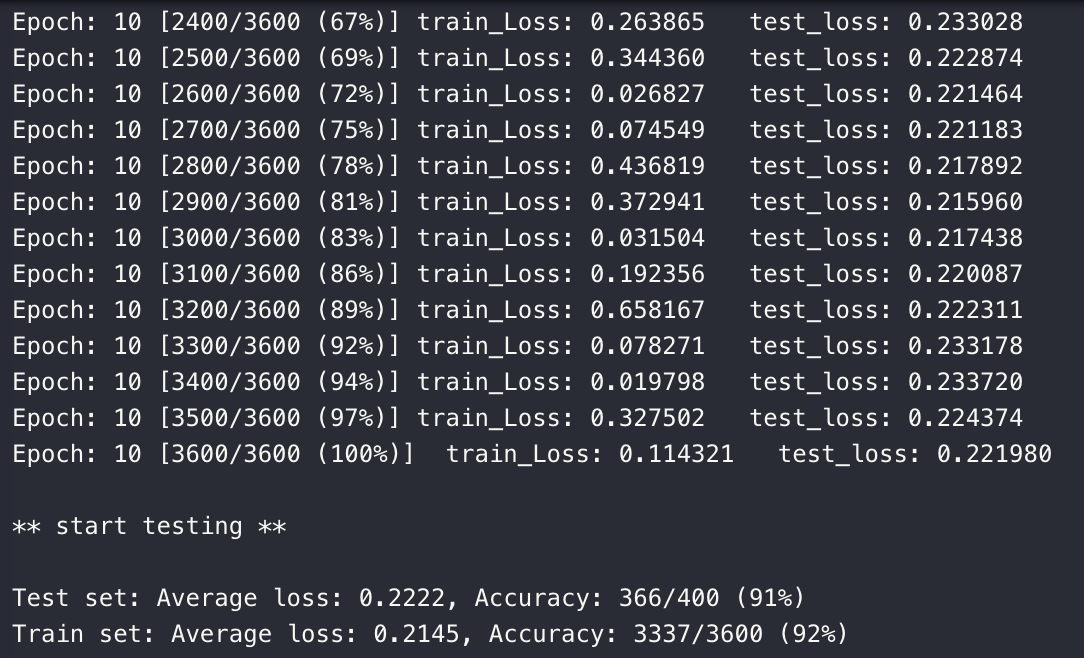
\includegraphics[width = .5\textwidth]{result3}
    \caption{Classification result}
    \label{res3}
\end{figure}

The train loss and test loss after each input of the mini batch is as shown in $\ref{loss3}$
\begin{figure}[htbp]
    \centering
    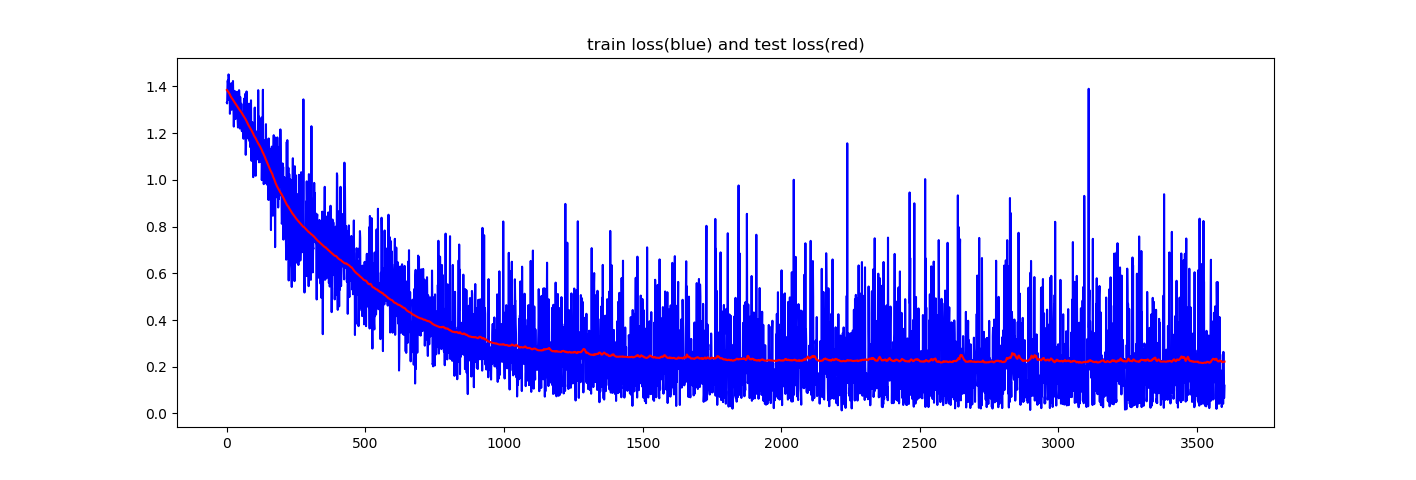
\includegraphics[width = \textwidth]{loss3}
    \caption{ }
    \label{loss3}
\end{figure}

\section{Regression}

The network is shown in $\ref{net2}$, each hidden layer has 20 tanh nodes,
\begin{figure}[htbp]
    \centering
    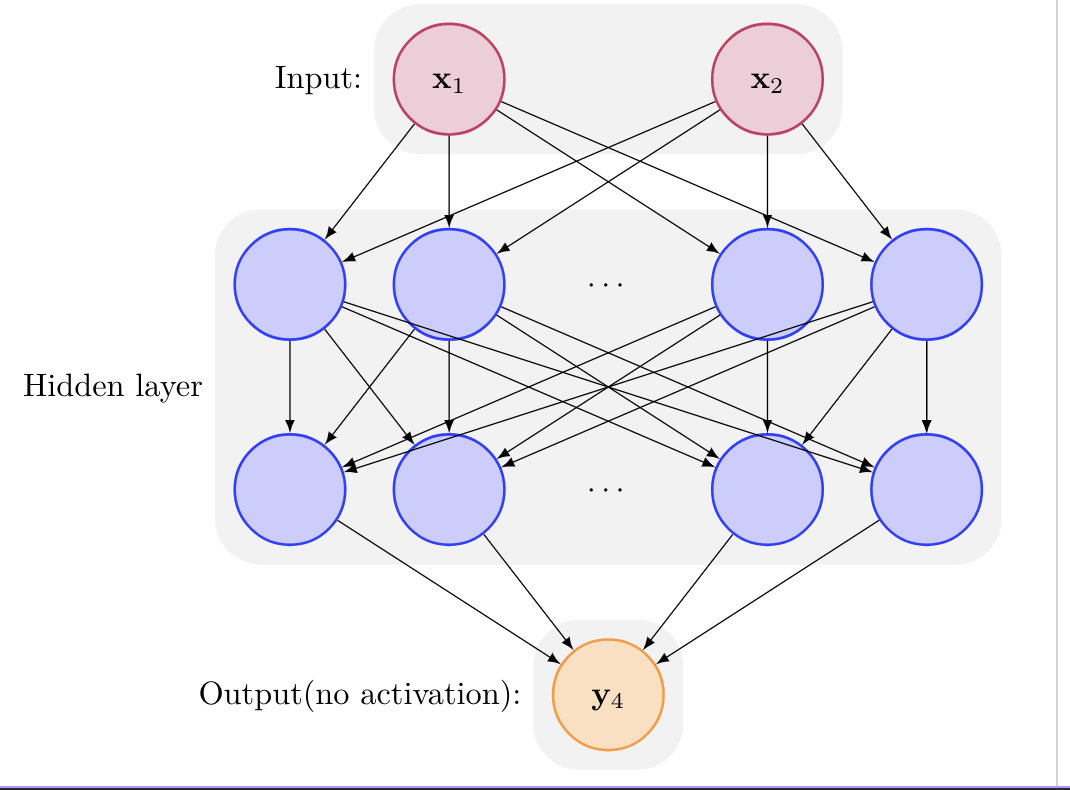
\includegraphics[width = .65\textwidth]{net2}
    \caption{fc-net-2}
    \label{net2}
\end{figure} 

Data samples are uniformly generated from [$-10, 10]\times[-10, 10]$ plane, since x and y is independent, we can genrate them respectively.
Using Adam and gradient clipping (the loss is extremely large), after 150 training epoch we get the loss evolution curves in $\ref{loss4}$.

\begin{figure}[htbp]
    \centering
    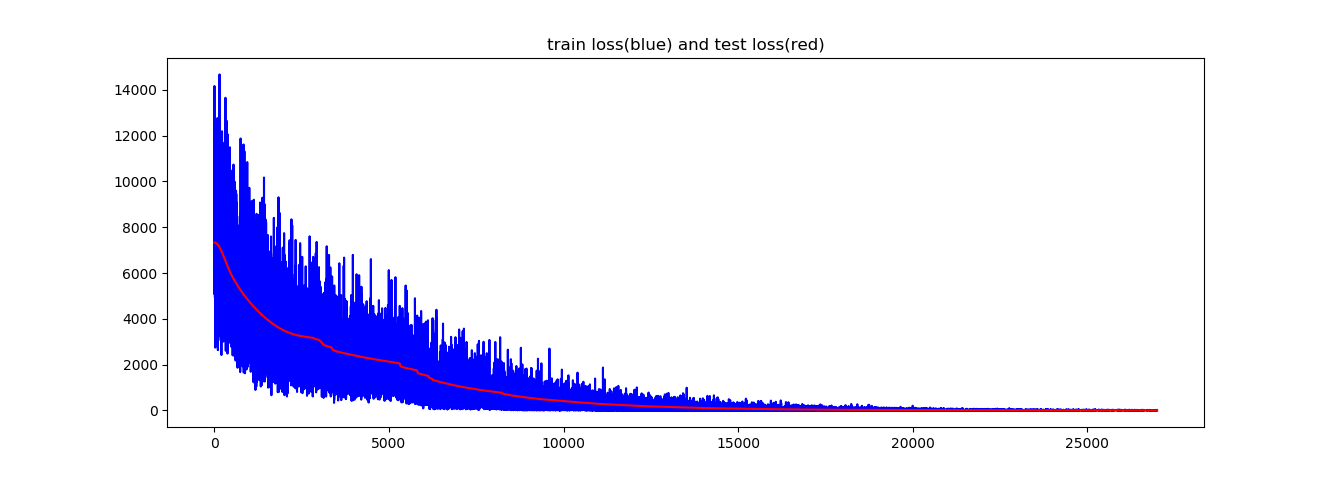
\includegraphics[width = \textwidth]{loss4}
    \caption{ }
    \label{loss4}
\end{figure}

The final train and test loss are shown in $\ref{res4}$.

\begin{figure}[htbp]
    \centering
    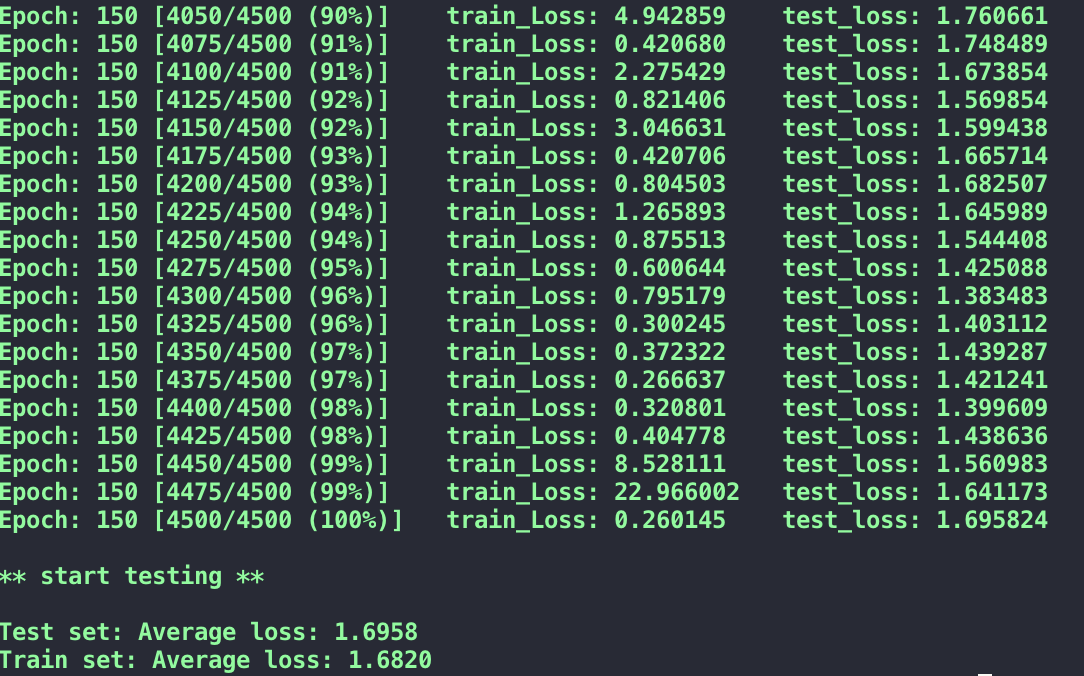
\includegraphics[width = .7\textwidth]{result4}
    \caption{Regression result}
    \label{res4}
\end{figure}

To intuitively show the fit, first we show the data samples in $\ref{data4}$

\begin{figure}[htbp]
    \centering
    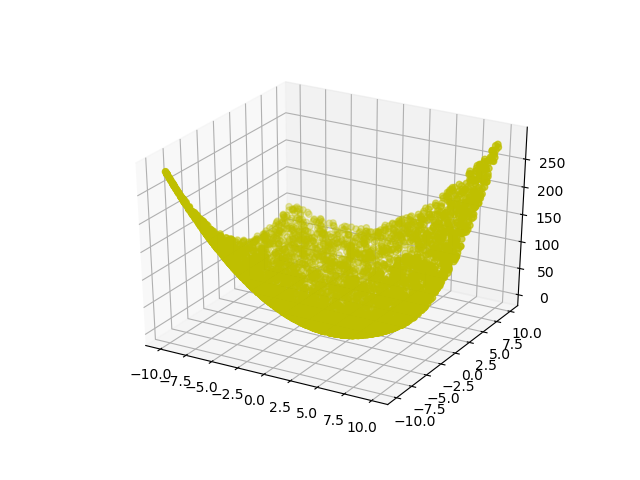
\includegraphics[width = .7\textwidth]{data4}
    \caption{data samples}
    \label{data4}
\end{figure}

The model output fit is shown in $\ref{fit4}$

\begin{figure}[htbp]
    \centering
    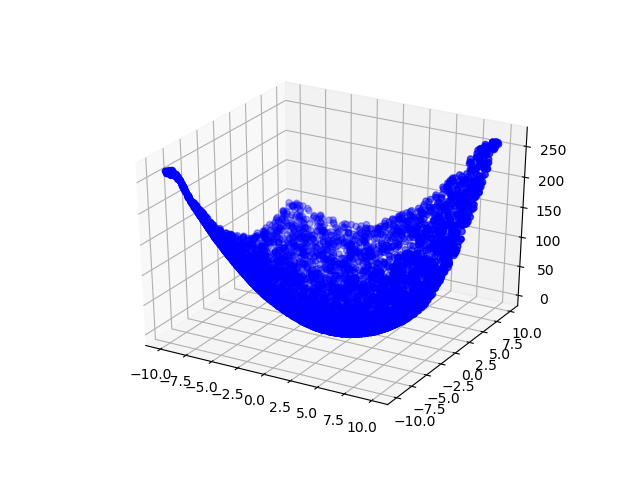
\includegraphics[width = .7\textwidth]{fit4}
    \caption{model fit}
    \label{fit4}
\end{figure}



\section{CNN}

In MNIST there are 60000 training samples and 10000 test samples, take as required randomly $10\%$ of the training samples as training set and randomly $10\%$ 
of the test samples as test set, one can leverage CNN and F-C to train a network that recognizes if the 2 input images represent the same digit or not, but mutually
combining elements of the whole dataset is time and memory costly, an easy way to do this is given an index when training, generating a random pair from either the same label set
or the complementary label sets, and when it comes to testing, randomly generating positive or negative pair from MNIST.test\_data, thus the dataset is modified to tackle
the learning task.

The architecture is as follows:
\begin{itemize}
    \item Input: $batch\_size \times 2 \ plane\ counts \times Height \times Width$
    \item Convolutional layer: channels: $2 \to 20$, kernel: $5\times5$, stride: $1 \times 1$
    \item Relu
    \item Maxpooling: $2\times 2$
    \item Convolutional layer: channels: $20 \to 40$, kernel: $5\times5$, stride: $1 \times 1$
    \item Relu
    \item Maxpooling: $2\times 2$
    \item Flattening(3D to 1D): $40 \times 4 \times 4 \to 640$
    \item Full-connected layer: $640 \to 20$
    \item Relu
    \item Full-connected layer: $20 \to 1$
    \item Sigmoid 
    \item Binary cross entropy loss
\end{itemize}

I used ADAM as its optimizer in order to make it converge faster.

In the first place, I tried 30 epochs, $\ref{loss5}$ demonstrates the train and test loss curves.
\begin{figure}[htbp]
    \centering
    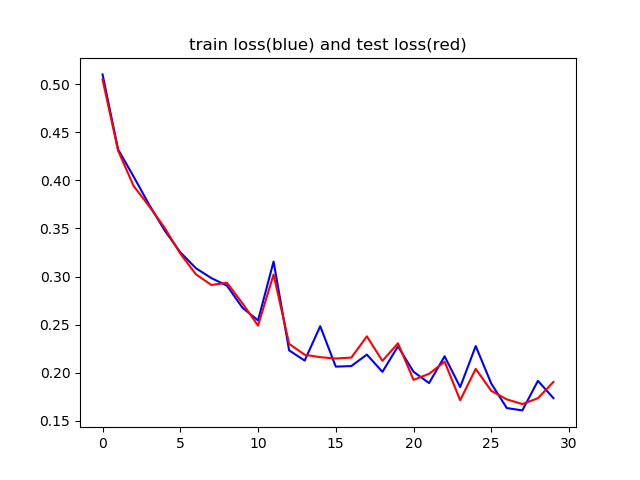
\includegraphics[width = \textwidth]{loss5}
    \caption{learning curve}
    \label{loss5}
\end{figure}

The final evaluation $\ref{res51}$:
\begin{figure}[htbp]
    \centering
    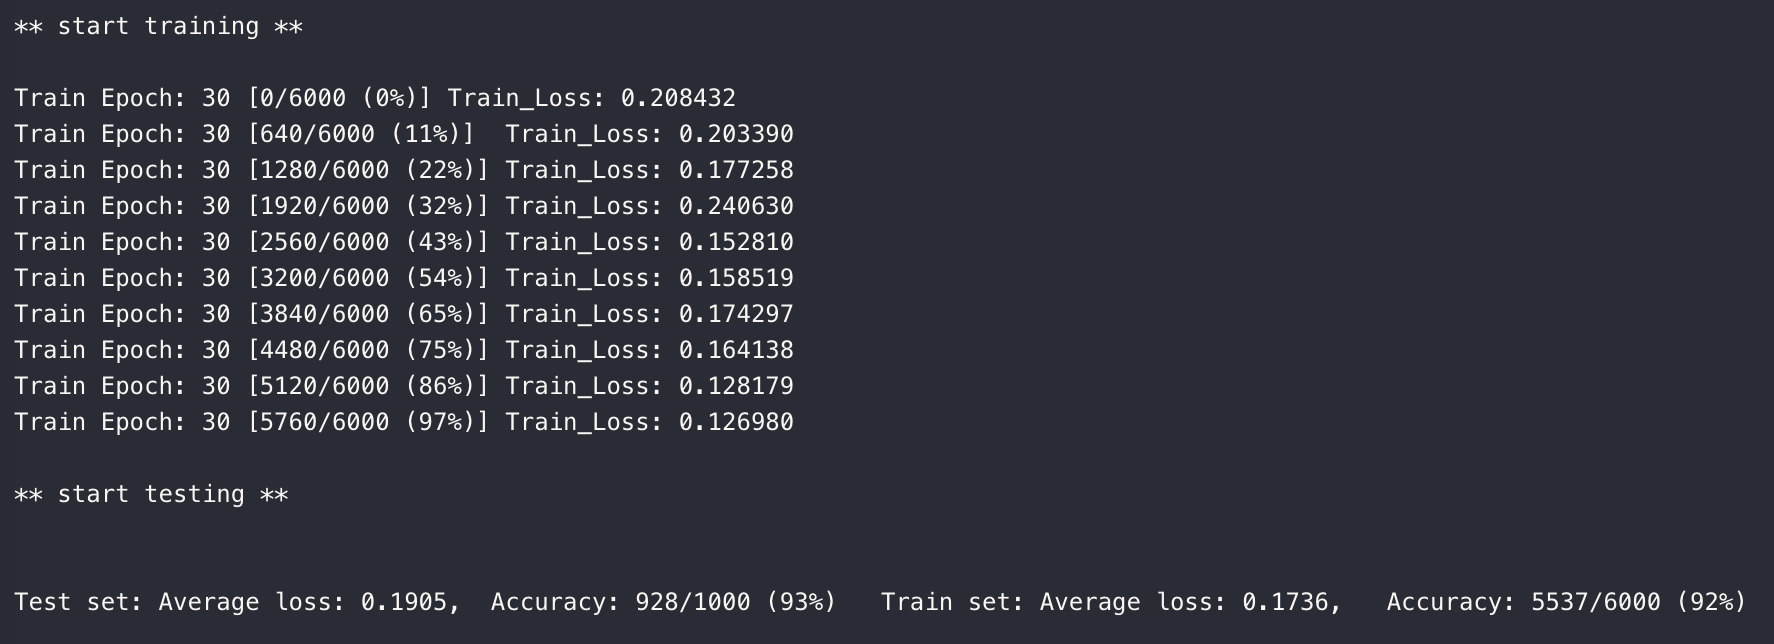
\includegraphics[width = \textwidth]{res51}
    \caption{}
    \label{res51}
\end{figure}

Continue training, the score will be higher, after 300 epochs,(fairly long time in my laptop)
I get $\ref{res52}$, while the loss evolution is as shown in $\ref{loss52}$
\begin{figure}[htbp]
    \centering
    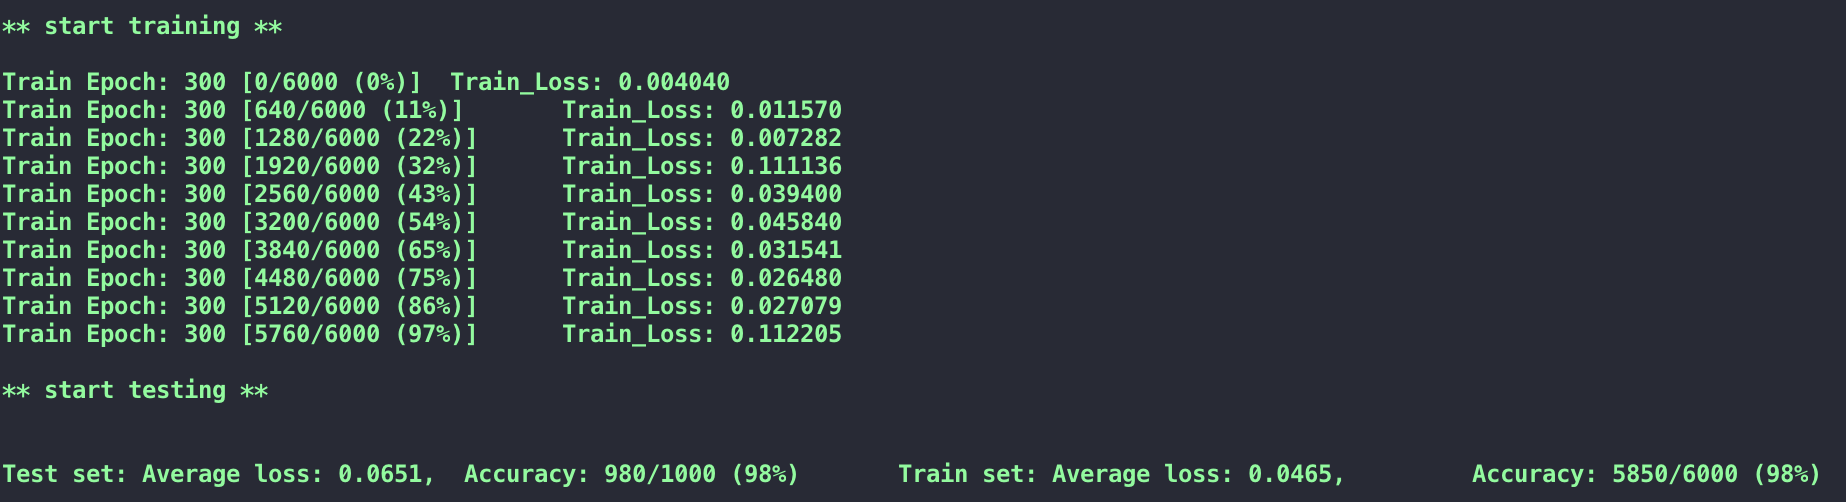
\includegraphics[width = \textwidth]{res52}
    \caption{}
    \label{res52}
\end{figure}

\begin{figure}[htbp]
    \centering
    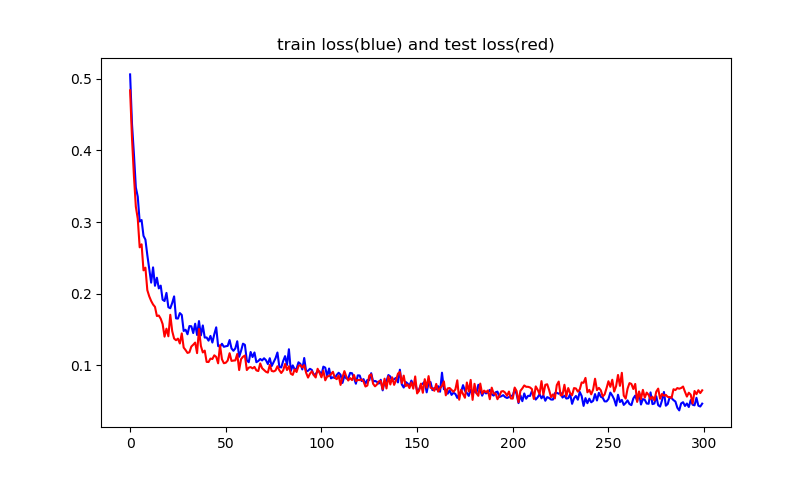
\includegraphics[width = \textwidth]{loss52}
    \caption{loss evolution}
    \label{loss52}
\end{figure}
Note that the accuracy improvement is slow, and has been stuck in $98\%$ after 230 epochs.


\end{document}